\documentclass{beamer}

\usetheme{Madrid}

\usepackage{etoolbox,refcount}
\usepackage{multicol}

\newcounter{countitems}
\newcounter{nextitemizecount}
\newcommand{\setupcountitems}{%
  \stepcounter{nextitemizecount}%
  \setcounter{countitems}{0}%
  \preto\item{\stepcounter{countitems}}%
}
\makeatletter
\newcommand{\computecountitems}{%
  \edef\@currentlabel{\number\c@countitems}%
  \label{countitems@\number\numexpr\value{nextitemizecount}-1\relax}%
}
\newcommand{\nextitemizecount}{%
  \getrefnumber{countitems@\number\c@nextitemizecount}%
}
\newcommand{\previtemizecount}{%
  \getrefnumber{countitems@\number\numexpr\value{nextitemizecount}-1\relax}%
}
\makeatother    
\newenvironment{AutoMultiColItemize}{%
\ifnumcomp{\nextitemizecount}{>}{3}{\begin{multicols}{2}}{}%
\setupcountitems\begin{itemize}}%
{\end{itemize}%
\unskip\computecountitems\ifnumcomp{\previtemizecount}{>}{3}{\end{multicols}}{}}


\usepackage{siunitx}
\usepackage{amsmath}
\usepackage{amsfonts}
\usepackage{amssymb}
\usepackage{array}
\newcolumntype{L}[1]{>{\raggedright\let\newline\\\arraybackslash\hspace{0pt}}m{#1}}
\newcolumntype{C}[1]{>{\centering\let\newline\\\arraybackslash\hspace{0pt}}m{#1}}
\newcolumntype{R}[1]{>{\raggedleft\let\newline\\\arraybackslash\hspace{0pt}}m{#1}}
\usepackage[utf8]{inputenc}
\usepackage[english]{babel}
\usepackage{url}
\usepackage{hyperref} 
\usepackage{float}
\usepackage{pgfplots}
\usepackage{tabularx,caption}
\usepackage{csvsimple}
\usepackage{listings,mdframed}
\usepackage{pifont}
\hypersetup{colorlinks =false}



\title{Optimization of LA in OLAP}

\subtitle{2nd general debriefing meeting}



\author{ Filipe Oliveira\ \and Sérgio Caldas}
% - Give the names in the same order as the appear in the paper.
% - Use the \inst{?} command only if the authors have different
%   affiliation.

%\institute[Universidade of Minho] % (optional, but mostly needed)
{
%  \{a57816\inst{1},a57779\inst{2}\}@alunos.uminho.pt
}
% - Use the \inst command only if there are several affiliations.
% - Keep it simple, no one is interested in your street address.
\date[UMinho, May 2016] % (optional)
  { \scriptsize \break \break \break \break 
\textbf{Advisors}: Alberto Proença and José Nuno Oliveira }

}

%\logo{\includegraphics[height=1.5cm]{lion-logo.png}}

\subject{Theoretical Computer Science}
% This is only inserted into the PDF information catalog. Can be left
% out. 

% If you have a file called "university-logo-filename.xxx", where xxx
% is a graphic format that can be processed by latex or pdflatex,
% resp., then you can add a logo as follows:

% \pgfdeclareimage[height=0.5cm]{university-logo}{university-logo-filename}
% \logo{\pgfuseimage{university-logo}}


% Let's get started
\begin{document}

\begin{frame}
  \titlepage
\end{frame}

\begin{frame}
\frametitle{Table of Contents}
\tableofcontents
\end{frame}

\section{Actual Progress}
\begin{frame}
\frametitle{Actual Progress}

\setbeamerfont{block body}{size=\footnotesize}

\begin{block}{Progress Until First Meeting}

\begin{itemize}
    \item LA Operations translated into our DSL
    \item Profiled the given dataset
    \item Our approach decisions
    \begin{itemize}
        \item Use Sparse MKL Library
        \item Use Quarks structure from Glib library
        \item Use sparse matrices formats for matrices representations 
    \end{itemize}
\end{itemize}
\end{block}

\begin{block}{Progress Until Now}
\begin{itemize}
    \item Sequential version of LA Operations implemented and optimized
    \item Querie-1 translated into our DSL
    \item Querie-1 First Results in our HPC test environment
\end{itemize}
\end{block}
\end{frame}

\section{Translating TPC-H Query-1}
\begin{frame}[fragile]
\frametitle{Translating TPC-H Query-1}

\begin{block}{TPC-H Query-1 (simplified)}
\begin{lstlisting}[
           language=SQL,
           showspaces=false,
           basicstyle=\footnotesize,
           %numbers=left,
           numberstyle=\tiny,
           commentstyle=\color{gray}
        ]
SELECT l_returnflag, l_linestatus,  sum(l_quantity)
FROM LINEITEM_1
WHERE l_shipdate >= '1998-08-28' AND l_shipdate <= '1998-12-01' 
GROUP BY l_returnflag, l_linestatus;
\end{lstlisting}
\end{block}

\\Translates into LA Operations:\par 

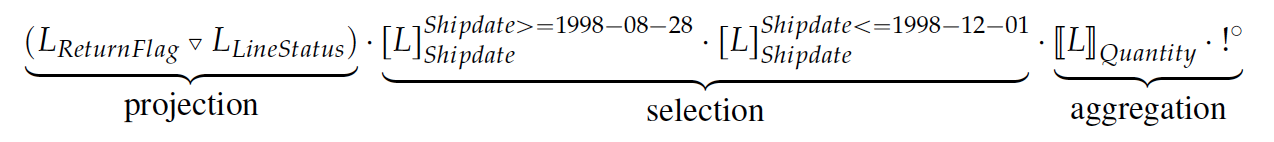
\includegraphics[width=\textwidth]{querie_1_la.png}

\end{frame}

\begin{frame}[fragile]
\frametitle{Translating TPC-H Query-1}

\\Translates into our DSL:\par 

\begin{figure}
    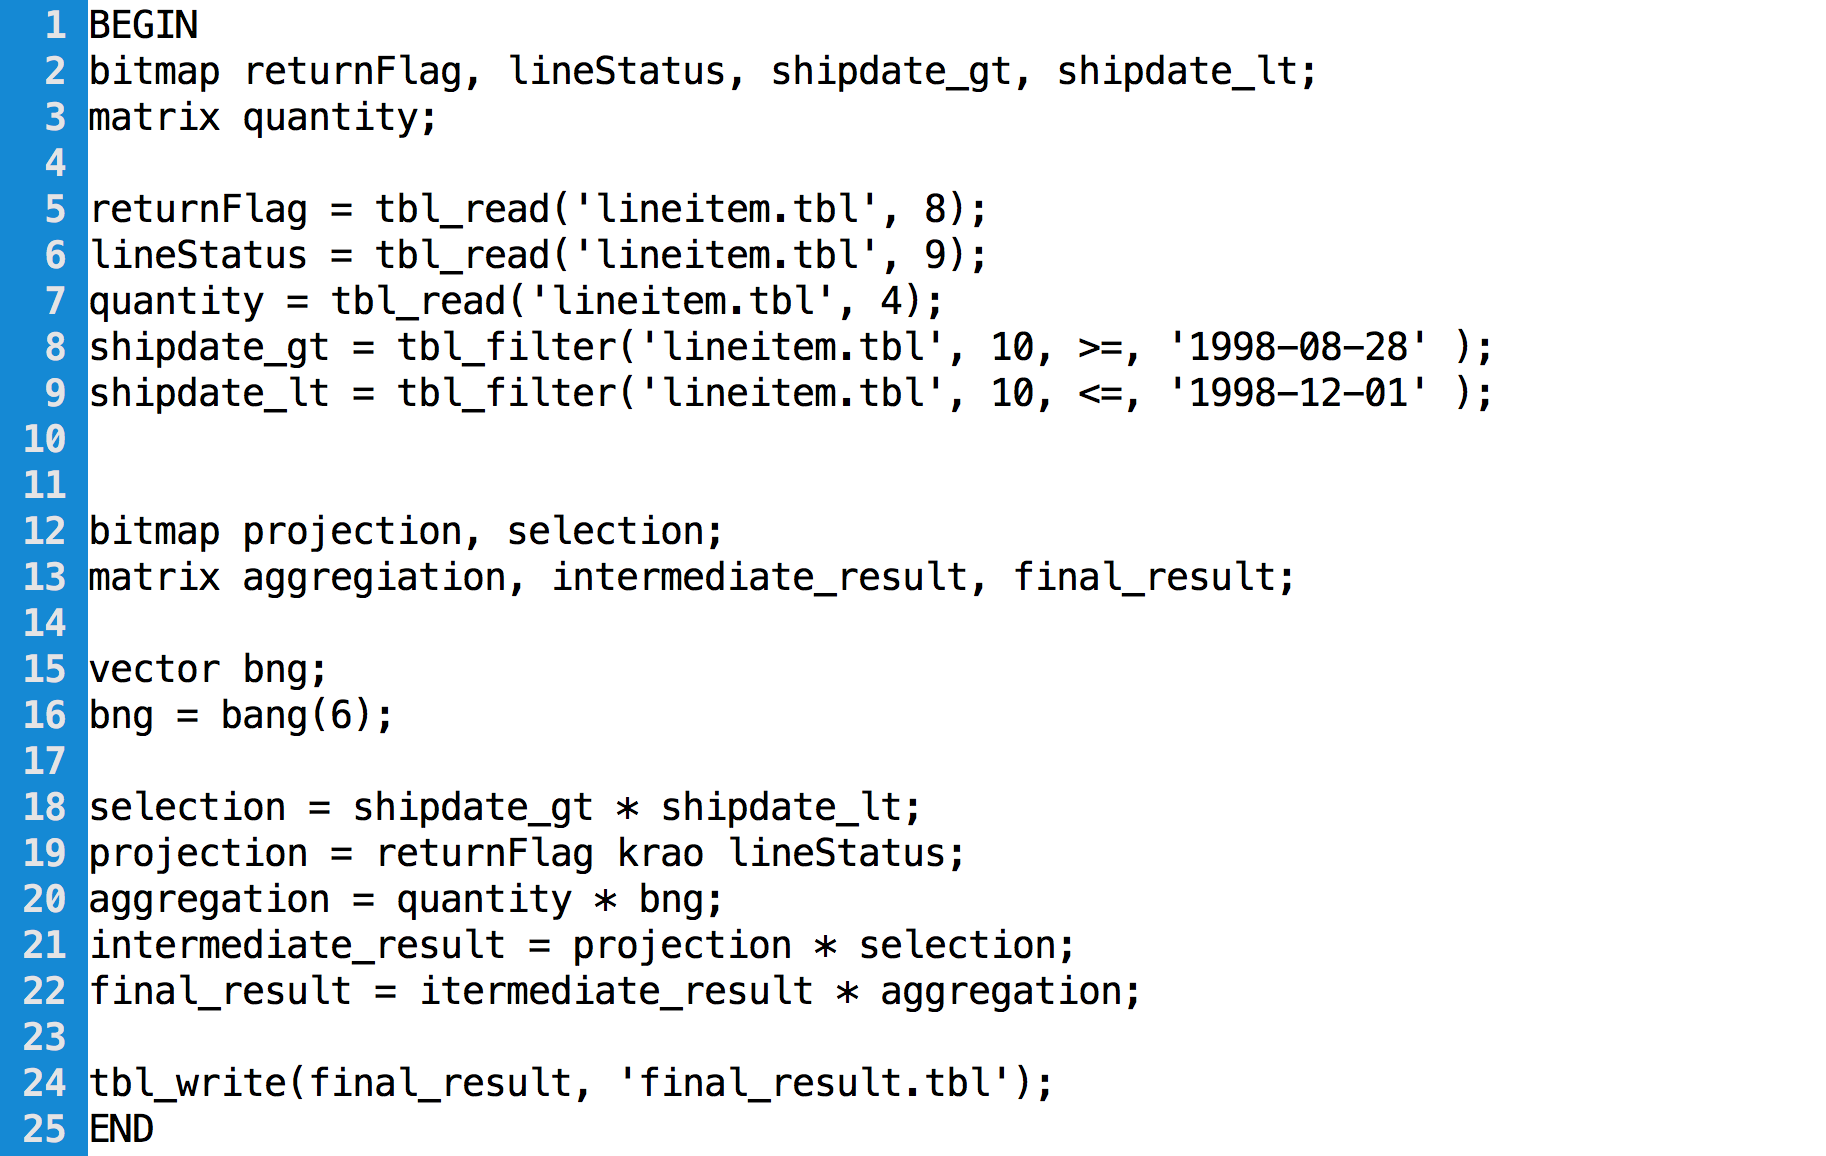
\includegraphics[width=0.95\textwidth,keepaspectratio]{querie-1.png}
\end{figure}


\end{frame}

\section{Implementing and optimizing the LA operations}
\begin{frame}[fragile]
\frametitle{Implementing and optimizing the LA operations}
\setbeamerfont{block body}{size=\footnotesize}

\begin{itemize}
    \item Several LA approaches were considered
        \vspace{0.3cm}
    \item La operations required: dot product, Kronecker Product, Hadamard Product, Khatri-Rao Product
    \vspace{0.5cm}
    \item Based on the special matrices property \textbf{(1 element per column)} all 4 products were simplified \textbf{(not enough to auto-vectorize)}
    \begin{itemize}
        \item All produced matrices have to be squared (if not pad with 0s)
    \end{itemize}
        \vspace{0.3cm}
        
        \item Opportunity
to use SSE/AVX vector instructions in all 3 products
        \begin{itemize}
            \item Enforced vectorization of loops % via #pragma simd
                    \vspace{0.25cm}

             \item All Data is aligned during creation accordingly to cache line size in order to assist vectorization % via (mkl_malloc) 
             \textbf{(Allocation alignment)}
                                 \vspace{0.25cm}

             
            \item Instructed the compiler to assume that all CSR arrays are aligned on an 32-byte boundary
                         \textbf{(Access alignment)}
% via  
            %%__assume_aligned

           
            


    \end{itemize}
\end{itemize}
\end{frame}

\begin{frame}[fragile]
\frametitle{Implementing and optimizing the LA operations}
\setbeamerfont{block body}{size=\footnotesize}

\begin{itemize}
    \item Khatri-Rao (used in query-1) optimization report:
\end{itemize}
\begin{figure}
    \centering
    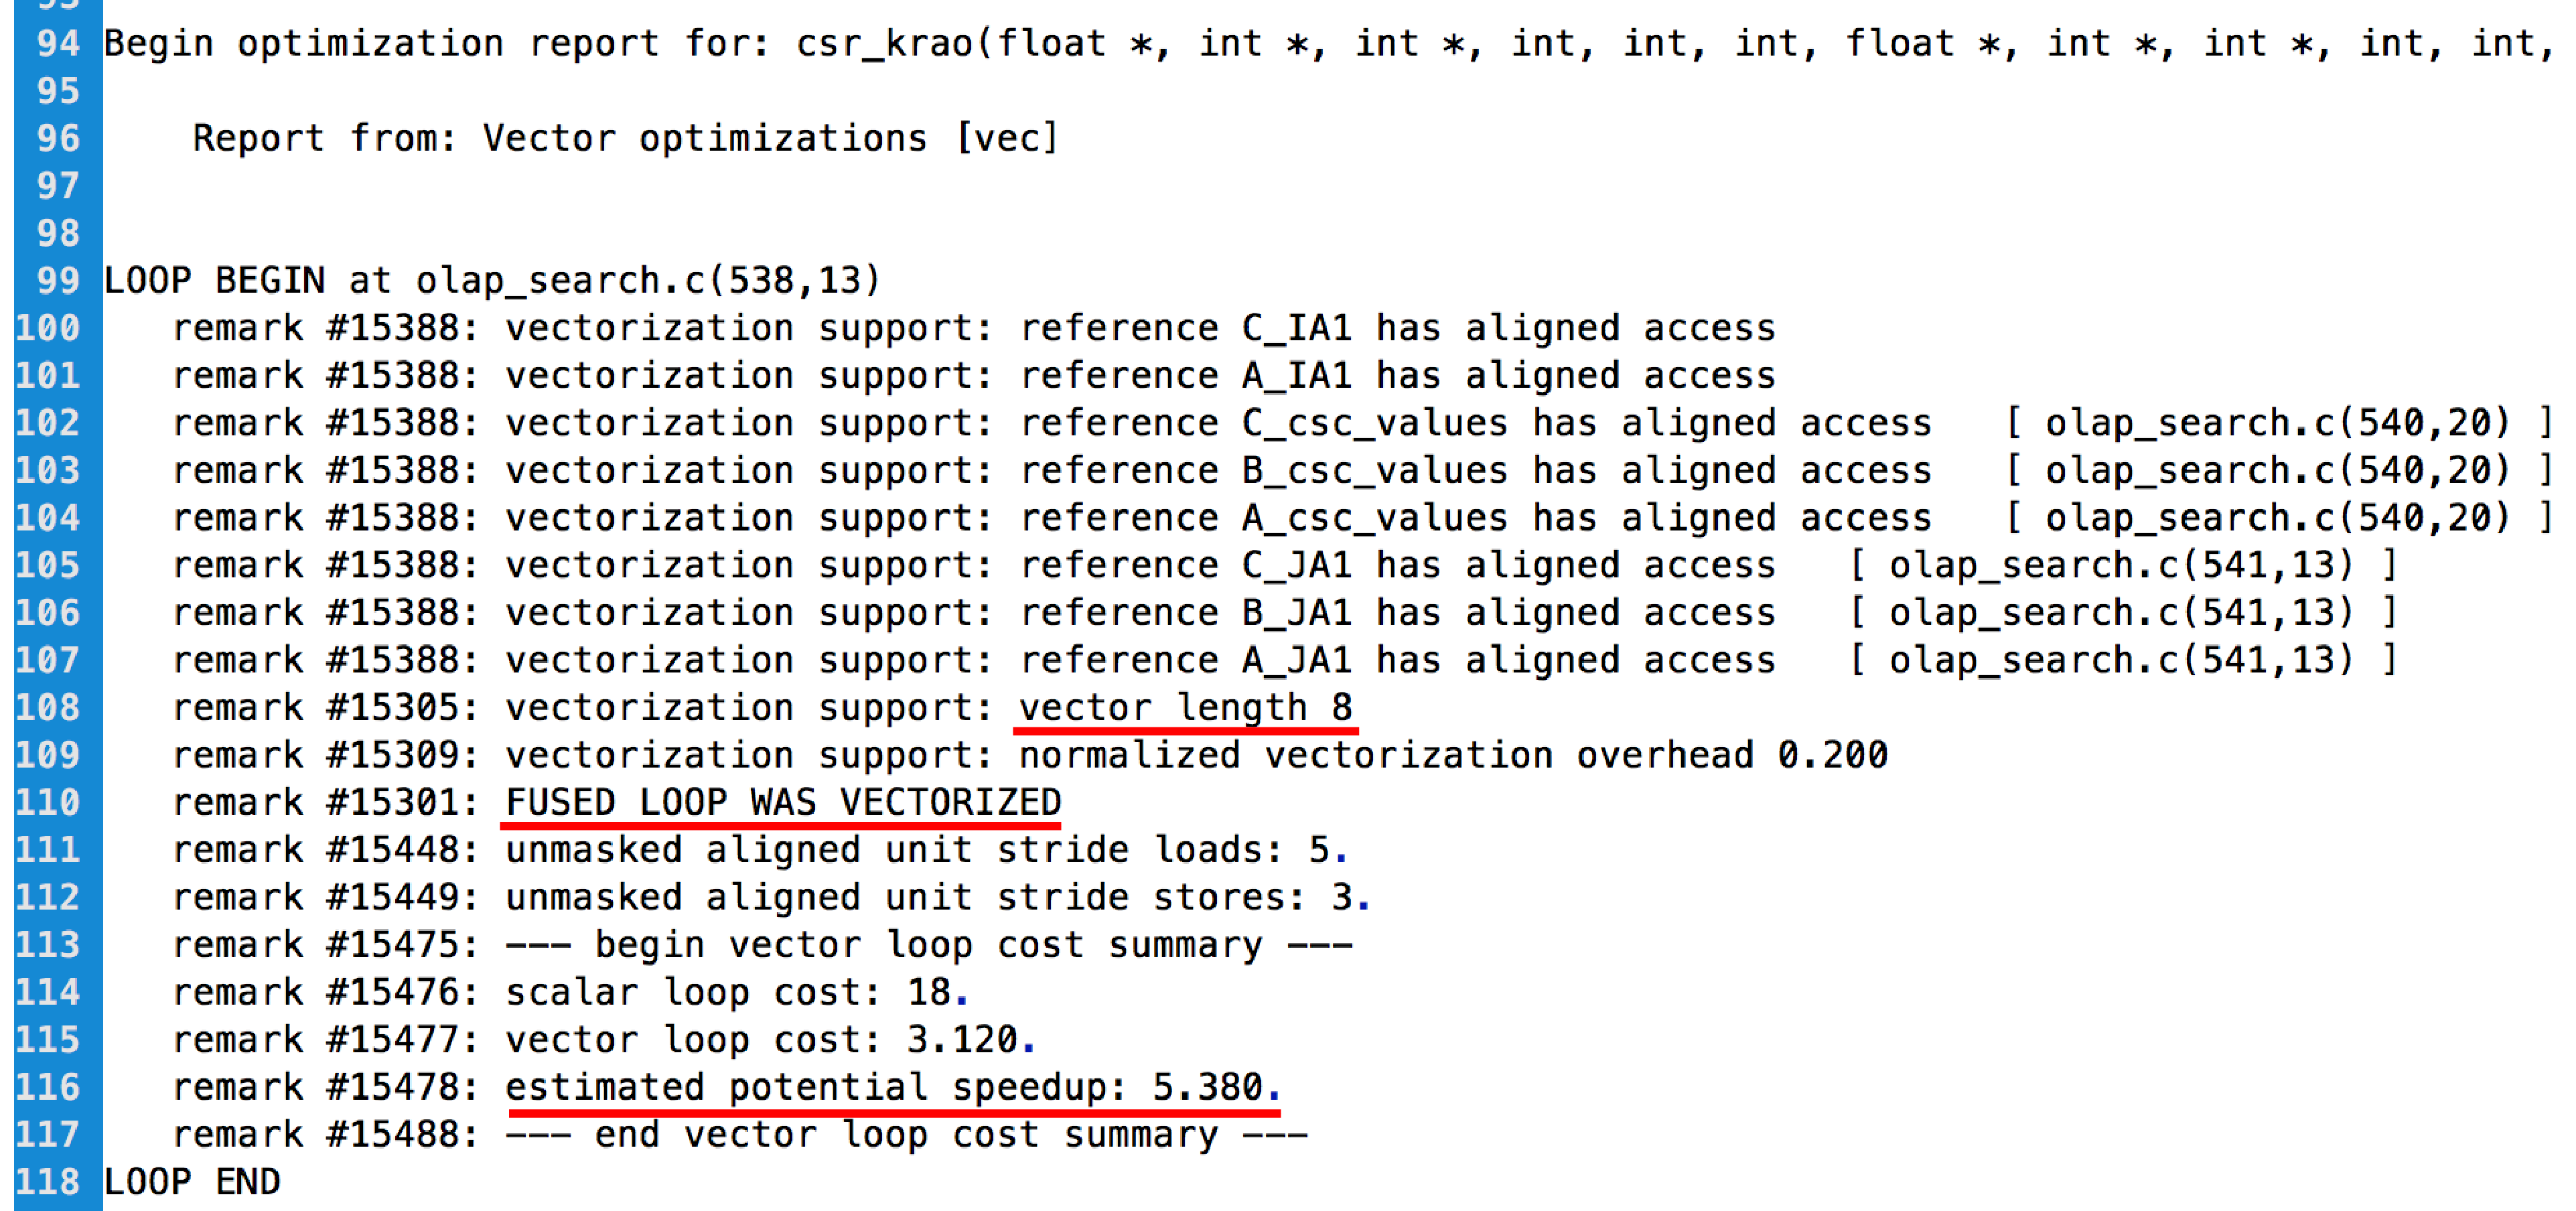
\includegraphics[width=0.95\textwidth,keepaspectratio]{krao_opt.png}
\end{figure}

\end{frame}

\section{Dataset Characterization}
\begin{frame}
\frametitle{Dataset Characterization}

\begin{block}{TPC-H Benchmark Tables}
    \begin{itemize}
    \item Used in TPC-H Querie-1: 
    \begin{AutoMultiColItemize}
                    \item \textbf{lineitem.tbl} 
  \end{AutoMultiColItemize}
        \vspace{0.3cm}
    \item Other TPC-H Benchmark Tables: 
    \begin{AutoMultiColItemize}
\item customer.tbl  
        \item nation.tbl  
        \item part.tbl      
        \item region.tbl
        \item orders.tbl    
        \item partsupp.tbl  
        \item supplier.tbl
  \end{AutoMultiColItemize}

    \end{itemize}
\end{block}

\begin{block}{Datasets}
    \begin{itemize}
        \item Generated data for different sizes: 1GB, 2GB, 4GB, 8GB, 16GB and 32 GB, producing 6 distinct LINEITEM DB tables. 
        \item To speed up queries, indexes were created for all DB Tables: 
        \begin{itemize}
            \item \small f.e.: CREATE INDEX l\_orderkey\_idx8 on LINEITEM\_8 (l\_orderkey); 
        \end{itemize}
    \end{itemize}
\end{block}

\end{frame}

\section{Test Platform}
\begin{frame}[fragile]
\frametitle{Environment Test Platform (Hardware)}

\setbeamerfont{block body}{size=\footnotesize}
\begin{table}[]
\small
\centering
  \begin{tabular}{ | L{5cm} | R{5cm} | }
  
    \hline
    System & compute-652-1 \\ 
    \hline 
    \# CPUs & 2 \\ 
    \hline
    CPU & Intel\textsuperscript{\textregistered} Xeon\textsuperscript{\textregistered} E5-2670v2	\\ \hline 
    Architecture & Ivy Bridge \\ 
    \hline 
    \# Cores per CPU & 10\\ 
    \hline 
    \# Threads per CPU & 20\\ 
    \hline 
    Clock Freq. & 2.5 GHz\\ 
    \hline 
    L1 Cache & 10 x 32 KB instruction caches \newline
    10 x 32 KB data caches\\ 
    \hline 
    L2 Cache & 2,560 KB \newline 256 KB per core\\ \hline 
    L3 Cache & 25 MB\\ 
    \hline 
    Inst. Set Ext. & AVX, SIMD\\ 
    \hline 
    \#Memory Channels & 4 \\ 
    \hline 
    Vendors Announced Peak Memory BW & 59.7 GB/s \\ \hline
    Measured Peak Memory BW & 57.18 GB/s \\
    \hline
  \end{tabular}
     \label{table:characterization}
\end{table}

\end{frame}

\begin{frame}[fragile]
\frametitle{Environment Test Platform (Software)}

\setbeamerfont{block body}{size=\footnotesize}

\begin{itemize}
\item LA OLAP: 
    \begin{itemize}

    \item Compiler: ICC version 16.0.0 (GCC version 4.4.6 compatibility)
    \begin{itemize}
        \item no vectorization: -O3 -std=c99 -no-vec -farray-notation 
        \item vectorization: -O3 -std=c99 -farray-notation -xAVX -vec-report7
    \end{itemize}
    \item Intel\textsuperscript{\textregistered} MKL Version	11.3
    \begin{itemize}
        \item Link line: -lmkl\_intel\_lp64 -lmkl\_core -lmkl\_sequential -lpthread -lm
    \end{itemize}
        \end{itemize}

\vspace{0.35cm}
    \item PostgreSQL: version 9.6+ 
    \begin{itemize}
        \item Built with the following dependencies:
        \begin{itemize}
            \item GCC version 4.9.0
            \item Python 2.6.6
        \end{itemize}
        \item Why PostgreSQL 9.6+ ?
        \begin{itemize}
            \item Open-Source
            \item PostgreSQL has Parallel-Query available\footnotemark[1]
        \end{itemize}
    \end{itemize}
    \vspace{0.35cm}
    \item Benchmarking: 
    \begin{itemize}
        \item 22 TPC-H Benchmark  queries
        \end{itemize}
\end{itemize}

\tiny
\footnotetext[1]{\tiny http://www.postgresql.org/docs/9.6/static/runtime-config-resource.html}

\end{frame}



\section{Query-1 First Results}
\begin{frame}[fragile]
\frametitle{Query-1 First Results in our HPC test environment}
\setbeamerfont{block body}{size=\footnotesize}

\begin{figure}
    \centering
    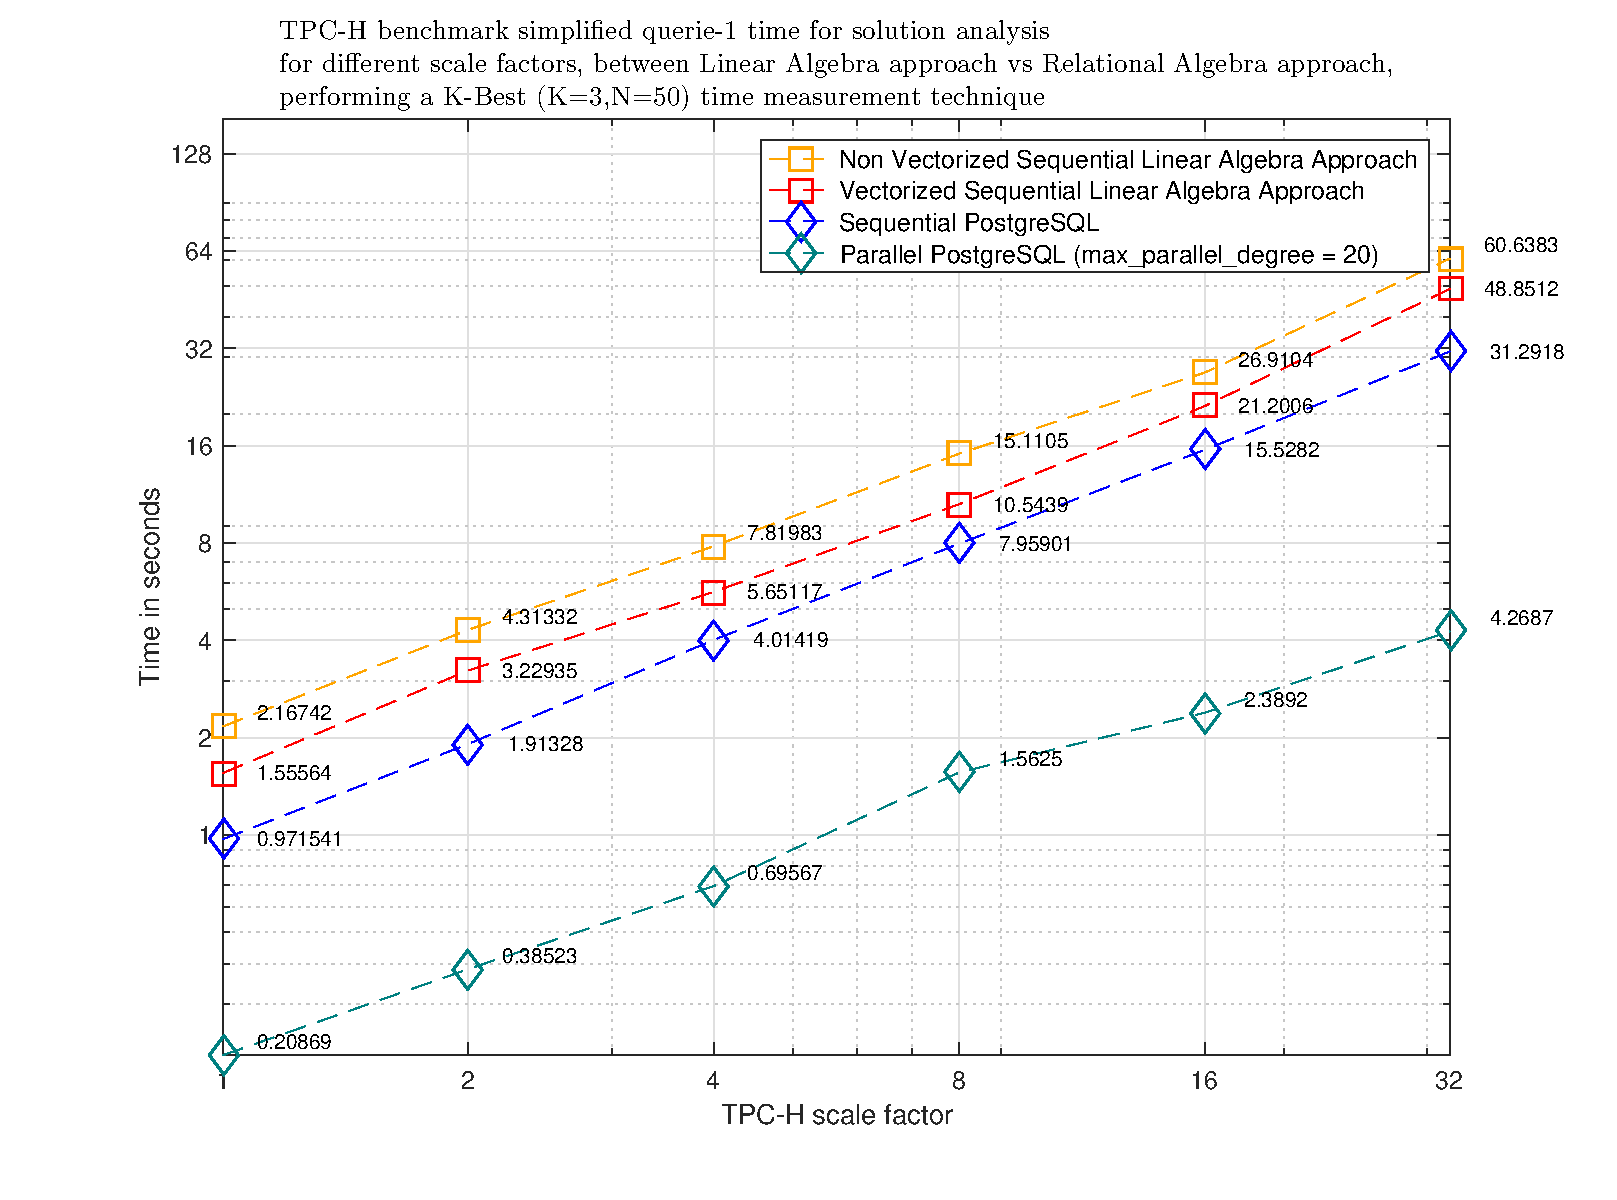
\includegraphics[width=0.92\textwidth,keepaspectratio]{TIME_LA_vs_RA.eps}
    \caption{Time OLAP vs PostgreSQL}
    \label{fig:olap_vs_postgresql}
\end{figure}

\end{frame}
\section{Next Steps}
\begin{frame}[fragile]
\frametitle{Planning our next steps}
\setbeamerfont{block body}{size=\footnotesize}

\begin{itemize}
    \item Multithreaded parallelism
    \begin{itemize}
        \item Expected high speedup values
    \end{itemize}
    \vspace{0.5cm}
    \item Improve data locality
    \begin{itemize}
    \item Implement all products in BSR format
            \item  Irregular access patterns decreases performance
    \end{itemize}
        \vspace{0.5cm}
    \item Analyse Gather/Scatter analysis for distributed memory parallelism
    \begin{itemize}
        \item Detect possible latency or bandwidth issues 
    \end{itemize}
\end{itemize}
\end{frame}

\begin{frame}
  \titlepage
\end{frame}

\end{document}


